% Document packages / layout
\documentclass[12pt]{article}

% --------------------------------------------------------------
% Abhi's Standard math Preamble.
% --------------------------------------------------------------

% Beauty Packages
\usepackage[margin=1in]{geometry} %1 inch margins
\usepackage{color}
\usepackage[final]{microtype}
\emergencystretch=1em

%% Linking Packages
\PassOptionsToPackage{hyphens}{url}
%\usepackage[plainpages=false, colorlinks=true, allcolors=red]{hyperref}
\usepackage[plainpages=false, allcolors=red]{hyperref}

% Math Packages
\usepackage{amsmath,amsthm,amssymb}
\usepackage{commath} %for \norm and \abs
\usepackage{bm}
\usepackage{dsfont}
\usepackage{mathtools}
\usepackage{mathrsfs}
\usepackage{physics}
\usepackage{stmaryrd}
\usepackage{xfrac}
\allowdisplaybreaks

% Quality of Life Packages
\usepackage{enumitem} %styles of enumeration
\usepackage{ulem} %strikethrough
\usepackage{pgffor}
\usepackage{booktabs} %Better quality tables
\usepackage{float} %H option for figures

% Bibliography Packages
\usepackage[backend=biber, style=alphabetic]{biblatex}
\addbibresource{citations.bib}
\usepackage{breakcites}

% Aliases and Package Settings
%% Operator aliases
\newcommand{\mc}[1]{\mathcal{#1}}
\newcommand{\mb}[1]{\mathbb{#1}}
%% Set aliases
\newcommand{\C}{\mathbb{C}}
\newcommand{\N}{\mathbb{N}}
\newcommand{\Z}{\mathbb{Z}}
\newcommand{\Q}{\mathbb{Q}}
\newcommand{\R}{\mathbb{R}}
%% analysis aliases
\newcommand{\e}{\varepsilon}
\DeclarePairedDelimiterX{\inp}[2]{\langle}{\rangle}{#1, #2}
%% Matrix aliases
\newcommand{\T}{\mathrm{T}}
\renewcommand{\vec}[1]{{\mathchoice
                     {\mbox{\boldmath$\displaystyle{#1}$}}
                     {\mbox{\boldmath$\textstyle{#1}$}}
                     {\mbox{\boldmath$\scriptstyle{#1}$}}
                     {\mbox{\boldmath$\scriptscriptstyle{#1}$}}}}
\newcommand{\mat}[1]{\mathbf{{#1}}}
% Chertock aliases
\newcommand*\xbar[1]{%
  \hbox{%
    \vbox{%
      \hrule height 0.5pt % The actual bar
      \kern0.15em%         % Distance between bar and symbol
      \hbox{%
        \kern-0.1em%      % Shortening on the left side
        \ensuremath{#1}%
        \kern-0.0em%      % Shortening on the right side
      }%
    }%
  }%
}


\begin{document}
\title{
  A Well-Balanced Stochastic Galerkin Method for PDEs with Random Forcing
}
\author{%
  Abhijit Chowdhary\footnote{%
    Department of Mathematics, North Carolina State University, Raleigh, NC
    27695, USA (\url{achowdh2@ncsu.edu}, \url{ajshedlo@ncsu.edu})
  }\ \ 
  and Andrew Shedlock\footnotemark[1]
}
\date{Last Edited: \today}
\maketitle
\tableofcontents

\clearpage

%%%%%%%%%%%%%%%%%%%%%%%%%%%%%%%%%%%%%%%%%%%%%%%%%%%%%%%%%%%%%%%%%%%%%%%%%%%%%%%%
%%% Introduction
%%%%%%%%%%%%%%%%%%%%%%%%%%%%%%%%%%%%%%%%%%%%%%%%%%%%%%%%%%%%%%%%%%%%%%%%%%%%%%%%
\section{Introduction}



\cite{Jin2015}


%%%%%%%%%%%%%%%%%%%%%%%%%%%%%%%%%%%%%%%%%%%%%%%%%%%%%%%%%%%%%%%%%%%%%%%%%%%%%%%%
%%% Methods
%%%%%%%%%%%%%%%%%%%%%%%%%%%%%%%%%%%%%%%%%%%%%%%%%%%%%%%%%%%%%%%%%%%%%%%%%%%%%%%%
\section{Methods}
As we described in the introduction, the scheme we will be working with combines parts of a well-balanced scheme and stochastic galerkin method. As we are working a system of the form
\begin{align}
    u_t + f(u)_x &= -b'(x)u \label{PDE}
\end{align}
At the steady state we have that $u_t = 0$, and so $(\ref{PDE})$ becomes the steady state condition
\begin{align}
    f(u)_x +b'(x)u &= 0 \label{ss}
\end{align}
We will assume that our flux function $f$ is such that $\frac{f'(\xi)}{\xi}$ is a well-defined number for all $\xi$. We can now define an operator $D:\mathbb{R}\to\mathbb{R}$ by
\begin{align*}
    D(u) &= \int_0^{u}\frac{f'(\xi)}{\xi}d\xi
\end{align*}
Now if $u(x)$ is a strong solution to $\ref{ss}$ and $u > 0$, then by Liebniz rule
\begin{align*}
    D(u(x))_x + b'(x) &= \frac{f'(u(x))u_x}{u(x)} + b'(x) = \frac{f(u(x))_x}{u(x)} + b'(x) = 0
\end{align*}
This shows that if $u$ is a strong solution to $(\ref{ss})$ and $u > 0$, then $D(u(x)) + q(x)$ is equal to some constant. If we assume that $D$ is monotone so that $D'(x)\not=0$, then we can see that
\begin{align*}
    u(x) &= \frac{f(u)_x}{D'(x)}
\end{align*}
If we adopt the finite volume framework, then we shall have $N_x$ cells with uniform mesh size of $\Delta x$. For $j = 1, \ldots, N_x$, we let $x_j$ represent the point at the center of the cell and let $x_{j+1/2}$ represent the point at the cell interface. Since we will have a uniform mesh, then $\Delta x = x_{j+1/2}-x_{j-1/2}$. We also have a uniform discretization in time and let $t^n$ represent the discretization at then $n^{th}$ level and $\Delta t =t^{n}-t^{n-1}$. The cell average at $t^n$ over $[x_{j-1/2},x_{j+1/2}]$ is given by
\begin{align*}
    u_j^n &= \frac{1}{\Delta x}\int_{x_{j-1/2}}^{x_{j+1/2}} u(x,t^n)dx
\end{align*}
At the cell interfaces we will have
\begin{align*}
    D_{j+1/2} &= D(u_{j+1/2})\\
    f_{j+1/2} &= f(u_{j+1/2})\\
    b_{j+1/2} &= b(x_{j+1/2})
\end{align*}
Then discrete analog to $(\ref{ss})$ will be
\begin{align*}
    \frac{f_{j+1/2}- f_{j-1/2}}{\Delta x} &= -\frac{(b_{j+1/2}-b_{j-1/2})}{\Delta x}\Big(\frac{f_{j+1/2}-f_{j-1/2}}{D_{j+1/2}-D_{j-1/2}}\Big)\\
    D_{j+1/2}-D_{j-1/2} &= -(b_{j+1/2}-b_{j-1/2})\\
    D_{j+1/2}+b_{j+1/2} &= D_{j-1/2}+b_{j-1/2} = \text{constant}
\end{align*}
In particular for the Burgers' equation we have that $f(u) = \frac{u^2}{2}$, so $D(u) = u$ and so
\begin{align*}
    \frac{f_{j+1/2}-f_{j-1/2}}{D_{j+1/2}-D_{j-1/2}} &= \frac{u_{j+1/2}^2 - u_{j-1/2}^2}{2(u_{j+1/2}-u_{j-1/2})} = \frac{u_{j+1/2}+u_{j-1/2}}{2}
\end{align*}
It follows that the following semi-discrete method for the Burgers' equation is well-balanced. 
\begin{align}
    \partial_t u_j + \Big(\frac{u_{j+1/2}^2-u_{j-1/2}^2}{\Delta x}\Big) &= -\Big(\frac{b_{j+1/2}-b_{j-1/2}}{\Delta x}\Big)\Big(\frac{u_{j+1/2}+u_{j-1/2}}{2}\Big)\label{semidiscrete_burgers}
\end{align}
It is described in \cite{Jin2001} that for a general $f$ that the scheme is well balanced. 
\begin{align}
    \partial_t u_j + \Big(\frac{f_{j+1/2}-f_{j-1/2}}{\Delta x}\Big) &= -\Big(\frac{b_{j+1/2}-b_{j-1/2}}{\Delta x}\Big)\Big(\frac{u_{j+1/2}+u_{j-1/2}}{2}\Big) \label{deterministic_wb}
\end{align}
In particular, $(\ref{semidiscrete_burgers})$ is a special case of this general formulation. This gives us the formulation for the deterministic well-balancing.\\ \newline
For the stochastic case, we incorporate some uncertainty into our bottom topography via a random variable $Z:\Omega\to\mathbb{R}$ with law $P$. For every instance of our random variable $Z$, let $u(x,t;Z)$ be the function $(x,t)\to u(x,t;Z)$ which solves
\begin{align} \label{Stochastic_PDE}
    u_t(x,t;Z) + f(u(x,t;Z))_x &= - b(x;Z)u(x,t;Z)
\end{align}
If we suppose that we have appropriate integrability conditions so that $u(x,t;Z),Z\in L^2(P)$ holds for all $(x,t)$, then we can use that $u(x,t;Z)$ will be $Z-$measurable. Consider $$\mathcal{P}_Z = \{\phi(Z):\,\phi\,\,\text{is a polynomial of any order}\}$$ 
Then $\mathcal{P}_Z$ is a dense vector subspace in the space of all $Z-$measurable functions. Since $\mathcal{P}_Z\subset L^2(P)$ by our integrability assumption on $Z$ and that $L^2(P)$ is a Hilbert space, then we can find an orthonormal basis $\{\Phi_m(Z)\}_{m\in\mathbb{N}}$ of $\mathcal{P}_Z$. Thus $\{\Phi_m(Z)\}_{m\in\mathbb{N}}$ is dense in the space $Z-$measurable functions. Then since $u(x,t;Z)$ is $Z-$measurable, then we can find coefficients $\hat{u}_m(x,t)$ such that $P-$almost everywhere we have that
\begin{align*}
    u(x,t;Z) &= \sum_{m\in\mathbb{N}}\hat{u}_m(x,t)\Phi_m(Z)&&\hat{u}_m(x,t) = \mathbb{E}[u(x,t;Z)\Phi_m(Z)]\\
    b(x;Z) &= \sum_{m\in\mathbb{N}}\hat{b}_m(x)\Phi_m(Z)&&\hat{b}_m(x) = \mathbb{E}[b(x;Z)\Phi_m(Z)]\\
\end{align*}
We want our scheme to respect our stochastic PDE almost everywhere, this is equivalent to enforcing the condition
\begin{align}
    \mathbb{E}[(\partial_tu(x,t;Z) + f(u(x,t;Z))_x)\Phi_m(Z)] &= \mathbb{E}[-b'(x,Z)u(x,t;Z)\Phi_m(Z)] \label{stochastic_condition}
\end{align}
holds for all $m$. In the discrete setting, we can only take a finite number of basis elements, so let $N$ represent the number of nodes that we are considering. Then the galerkin approximation of $u$ and $b$ in terms of $Z$ is given by
\begin{align*}
    u_N(x,t;Z) &= \sum_{m=1}^{N+1}\hat{u}_m(x,t)\Phi_m(Z)\\
    b_N(x;Z) &= \sum_{m=1}^{N+1}\hat{b}(x)\Phi_m(Z)
\end{align*}
If we fix $t$, then let $u_{N,j} = u_N(x_j,t;Z)$ where the right hand side is the cell average over $[x_{j-1/2},x_{j+1/2}]$. We take $u_{j+1/2}\approx u_j$ and similarly for the other components to get that with $(\ref{deterministic_wb})$ we have that scheme
\begin{align*}
      \partial_t u_{N,j} + \Big(\frac{f(u_{N,j})-f(u_{N,j-1})}{\Delta x}\Big) &= -\Big(\frac{b_{N,j}-b_{N,j-1}}{\Delta x}\Big)\Big(\frac{u_{N,j}+u_{N,j-1}}{2}\Big) \label{deterministic_wb}
\end{align*}
If we then enforce the condition $(\ref{stochastic_condition})$, we derive the following condition on the scheme we construct
\begin{align}
    \mathbb{E}\Big[\Big(\partial_t u_{N,j} + \Big(\frac{f(u_{N,j})-f(u_{N,j-1})}{\Delta x}\Big)\Big)\Phi_m(Z)\Big] &= -\mathbb{E}\Big[\Big(\frac{b_{N,j}-b_{N,j-1}}{\Delta x}\Big)\Big(\frac{u_{N,j}+u_{N,j-1}}{2}\Big)\Phi_m(Z)\Big]\label{condition}
    \intertext{If we set $\bold{u}_j = (\hat{u}_{1,j},\ldots,\hat{u}_{N+1,j})^T$, define $E$ to be the tensor with components $e_{klm} = \mathbb{E}[\Phi_k\Phi_l\Phi_m]$ and $D$ to be the tensor with components $d_{klmnp} = \mathbb{E}[\Phi_k\Phi_l\Phi_m\Phi_n\Phi_p]$ and where $1\leq k,l,m,n,p\leq N+1$. We then define matrices $A_j,S,B$ to satisfy}
    A_{kl,j} &= \sum_{m=1}^{N+1}e_{klm}\hat{u}_{m,j}\nonumber\\
    B_{kl,j} &= \sum_{m=1}^{N+1}e_{klm}\hat{b}_{m,j}\nonumber\\
    S_{kl,j} &= \sum_{m,n,p=1}^{N+1}d_{klmnp}\hat{u}_{m,j}\hat{u}_{n,j}\hat{u}_{p,j}\nonumber
\end{align}
If $f(u) = \frac{u^2}{2}$, then a scheme which satisfies $(\ref{condition})$ and $(\ref{deterministic_wb})$ is
\begin{align*}
    \partial_t\bold{u}_j + \frac{A_j \bold{u}_j - A_{j-1}\bold{u}_{j-1}}{2\Delta x} &=- \frac{(B_j-B_{j-1})(\bold{u}_j + \bold{u}_{j-1})}{2\Delta x}
    \intertext{If $f(u) = \frac{u^4}{4}$, then a scheme which satisfies the stochastic condition and the well-balancing condition is}
    \partial_t\bold{u}_j + \frac{s_j \bold{u}_j - S_{j-1}\bold{u}_{j-1}}{4\Delta x} &=- \frac{(B_j-B_{j-1})(\bold{u}_j + \bold{u}_{j-1})}{2\Delta x}
\end{align*}
%%%%%%%%%%%%%%%%%%%%%%%%%%%%%%%%%%%%%%%%%%%%%%%%%%%%%%%%%%%%%%%%%%%%%%%%%%%%%%%%
%%% Results
%%%%%%%%%%%%%%%%%%%%%%%%%%%%%%%%%%%%%%%%%%%%%%%%%%%%%%%%%%%%%%%%%%%%%%%%%%%%%%%%
\section{Results}
In order to verify that the proposed methods satisfy the well-balanced claim, in this section we provide several numerical examples of it doing so.
Consider the stochastic PDE \eqref{Stochastic_PDE} that we constructed methods for last section; imposing the boundary conditions:
\[
\begin{cases}
    u(x,0) = 0, &\text{for } x > 0 \\
    u(0,t) = 2, &\text{for } t > 0
\end{cases}
\]
we solve the PDE under both Burger's flux $f(u) = u^2 /2$ and the alternate flux given by $f(u) = u^4 / 4$ over the following choices of bottom topography:
\begin{align}
    \label{b1}
    b_1(x,z)
    &=
    \begin{cases}
        (2+z) \cos(\pi x), & 4.5 \leq x \leq 5.5 \\
        0, & \text{otherwise}
    \end{cases} \\
    \label{b2}
    b_2(x,z)
    &=
    \begin{cases}
        0.1(2+z) \cos(\pi x), & 5 \leq x \leq 6 \\
        0, & \text{otherwise}
    \end{cases}
\end{align}
Bottom topography \eqref{b1} is continuous whereas \eqref{b2} is discontinuous, resulting in continuous and discontinuous resulting solutions.
In all examples $z \sim {\rm Uniform}[-1,1]$.

For all figures, we choose number of cells $N_c = 100$ and the time step is fixed to $\Delta t = 3200^{-1}$. 
In the steady state, assuming $u > 0$, \eqref{Stochastic_PDE} reduces down to $u'(x) = -b'(x,z)$, hence we find the steady state solution $u(x) = 2 - b(x,z)$, from which we can derive the steady state mean and standard deviation $\mathbb{E}[u] = 2 - 2b(x,0)$ and $\mathbb{V}[u] = \frac{1}{\sqrt{3}} |b(x,0)|$, which is what we compare the numerically computed solution to in Figures \ref{fig:b1-mean} - \ref{fig:b2-sd}.

\begin{figure}[!htb]
    \centering
    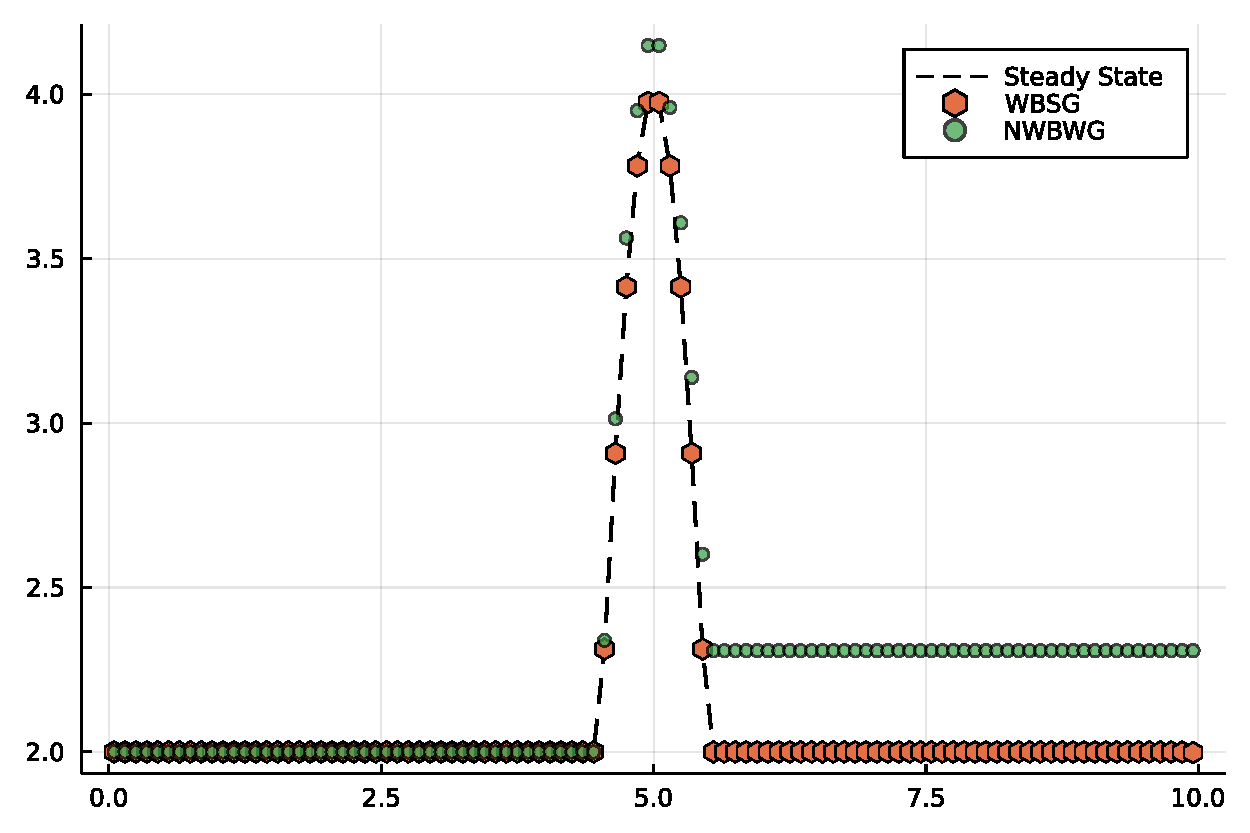
\includegraphics[width=0.75\textwidth]{Figures/mean_sgwb}
    \caption{Caption}
    \label{fig:b1-mean}
\end{figure}
\begin{figure}[!htb]
    \centering
    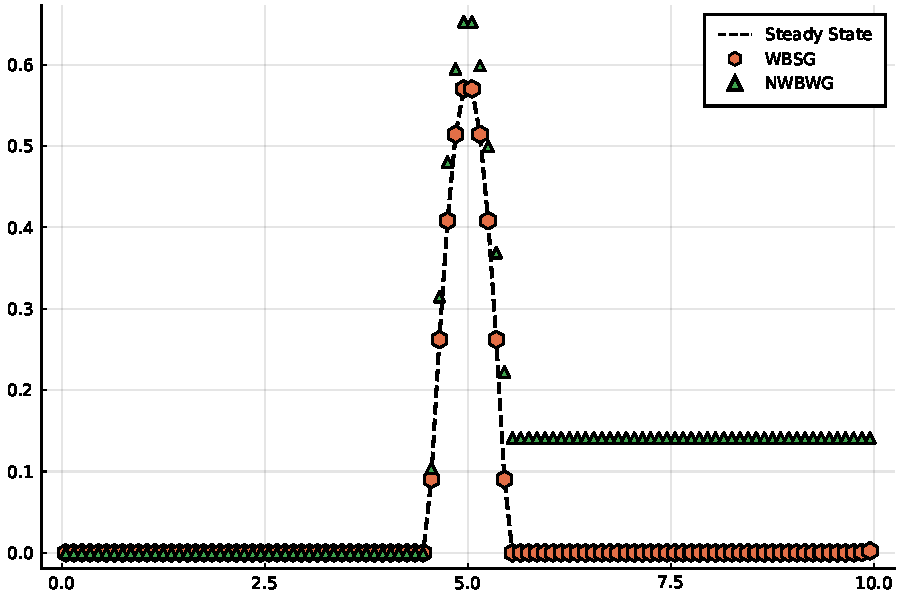
\includegraphics[width=0.75\textwidth]{Figures/sd_sgwb}
    \caption{Caption}
    \label{fig:b1-sd}
\end{figure}
\begin{figure}[!htb]
    \centering
    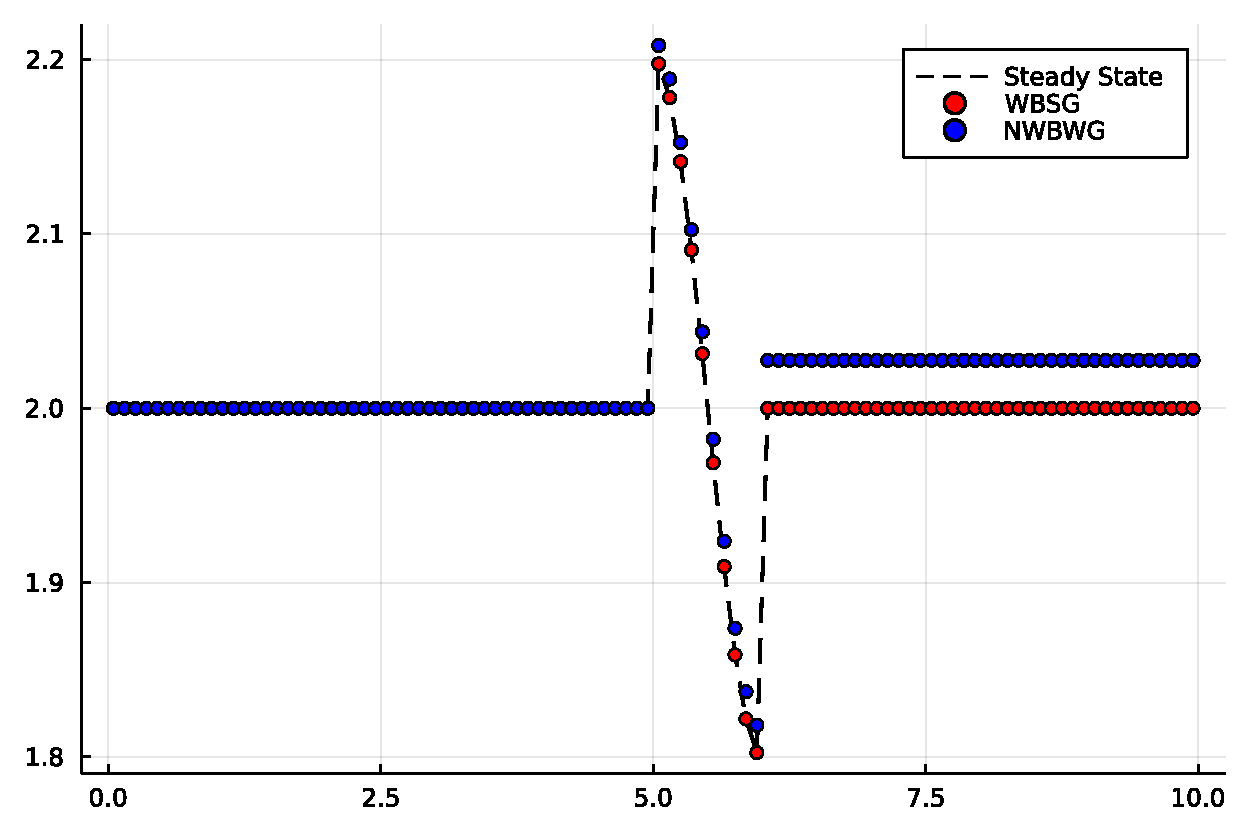
\includegraphics[width=0.75\textwidth]{Figures/mean_dc_sgwb}
    \caption{Caption}
    \label{fig:b2-mean}
\end{figure}
\begin{figure}[!htb]
    \centering
    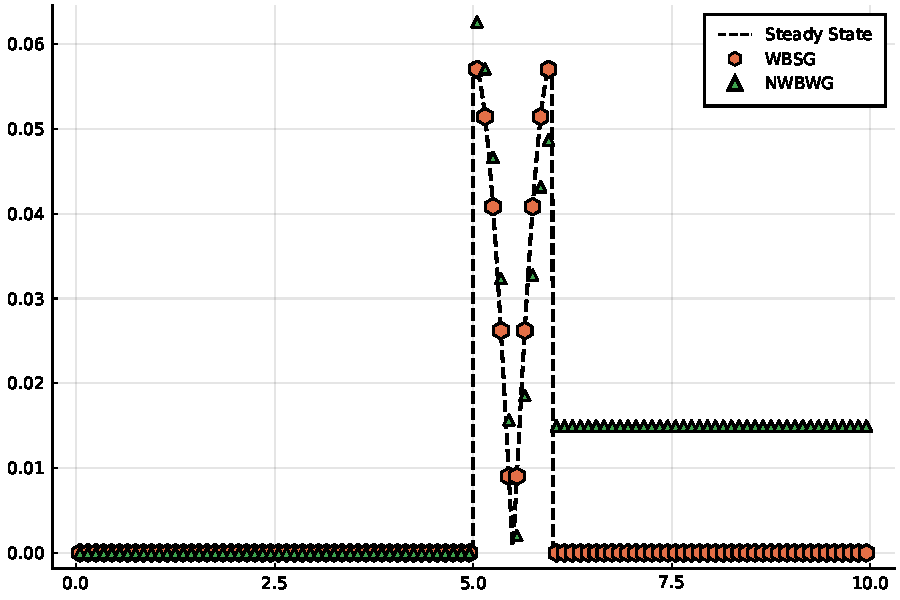
\includegraphics[width=0.75\textwidth]{Figures/sd_dc_sgwb}
    \caption{Caption}
    \label{fig:b2-sd}
\end{figure}


\begin{table}[!htb]
\centering
\begin{tabular}{@{}l|lll@{}}
\toprule
CPU Time & 100  & 200  & 400   \\ \midrule
1        & 2.83 & 3.62 & \ 7.28  \\
2        & 2.84 & 5.69 & 11.22 \\
3        & 3.14 & 6.07 & 12.22 \\
4        & 3.81 & 7.64 & 15.37 \\ \bottomrule
\end{tabular}
\caption{The estimated CPU time (seconds) for the Well-Balanced Stochastic Galerkin method for bottom topography $b_1$ and flux $f(u) = u^2/2$ with cell count $N_c \in \{100, 200, 400\}$ and number of gPC coefficients $M \in \{1,2,3,4\}$.}
\label{tab:cpu-time}
\end{table}


%%%%%%%%%%%%%%%%%%%%%%%%%%%%%%%%%%%%%%%%%%%%%%%%%%%%%%%%%%%%%%%%%%%%%%%%%%%%%%%%
%%% Conclusion
%%%%%%%%%%%%%%%%%%%%%%%%%%%%%%%%%%%%%%%%%%%%%%%%%%%%%%%%%%%%%%%%%%%%%%%%%%%%%%%%
\section{Conclusion}

%%%%%%%%%%%%%%%%%%%%%%%%%%%%%%%%%%%%%%%%%%%%%%%%%%%%%%%%%%%%%%%%%%%%%%%%%%%%%%%%
%%% References
%%%%%%%%%%%%%%%%%%%%%%%%%%%%%%%%%%%%%%%%%%%%%%%%%%%%%%%%%%%%%%%%%%%%%%%%%%%%%%%%
\printbibliography

\end{document}
